\documentclass[12pt]{article}

\usepackage[utf8]{inputenc}
\usepackage[english]{babel}
\usepackage{fancyhdr}
\usepackage{graphicx}
\graphicspath{ {./images/} }
\usepackage{titling}
\usepackage{wrapfig}
\usepackage{float}
\usepackage[table,xcdraw]{xcolor}
\usepackage{blindtext}
\usepackage{setspace}
\usepackage{listings}
\usepackage{tocloft}
\usepackage{placeins}
\usepackage[titletoc]{appendix}
\usepackage{etoolbox}
\usepackage{setspace}
\usepackage{makecell, caption}
\renewcommand\theadfont{\normalsize\bfseries\boldmath}
\usepackage{siunitx}
\sisetup{detect-weight, range-phrase=/, range-units = single}
\usepackage{lipsum}
\usepackage{amsmath,amssymb}
\usepackage{caption}
\usepackage{subcaption}
\usepackage{commath}
\usepackage{float}

\usepackage[T1]{fontenc}                
\usepackage{booktabs}

\usepackage[table,xcdraw]{xcolor}
\doublespacing
\usepackage[
    backend=biber,
    style=mla-new,
    citestyle=authoryear
    ]{biblatex}
\addbibresource{sources.bib}

\usepackage{geometry}
 \geometry{
 a4paper,
 left=25mm,
 right=25mm,
 bottom=25mm,
 top=25mm,
 }

\pagestyle{fancy}
\fancyhf{}
\chead{
         \textsc{Spoons, Curves, and an Evaluation of Cavalieri's Principle} 
    }
\rfoot{Page \thepage}

\begin{document}

\section{Introduction}

I love cooking: whether it's throwing a bunch of ingredients together and seeing what comes out or meticulously following a recipe for hours, it's something I love spending time doing. However, a major flaw I find in some recipes is that they tend to measure quantities by volume. There are standardised measurements in the US for a teaspoon and a tablespoon, but at home, I only have a standardised tablespoon. I usually end up approximating quantities in standardised teaspoons based on the teaspoons I own, but when creating complex desserts for example, even the smallest inaccuracies  can completely alter the textures and flavours. As a result, I've decided to investigate how the teaspoons I own actually compare to the US standard measurements so I can accurately follow recipes allowing me to create more complex dishes.

\section{Methodology}\label{method}

To mathematically find the volume of a shape, we can use integral calculus. However, upon inspection of my teaspoon, the shape of the volume bound appears to most closely resemble an elliptical paraboloid - meaning its shape is bound by two parabolas and an ellipse encapsulating it on top. 

As a result, this would involve multivariable calculus to solve, which is outside the scope of this investigation. Therefore, an alternative method to finding volume of irregular shapes, Cavalieri's Principle in three dimensions, will be the primary tool for this investigation. 

Cavalieri's Principle states that if two solids share the same cross sectional area when intersected by parallel planes and the same height, their volume will be the same as demonstrated below in Figure \ref{fig:cavasimp} (\citeauthor{cavalieri_1653}). Furthermore, this principle can be extended by creating hypothetical shapes, which can provide visually intuitive solutions to find the volume of more complex shapes (Figure \ref{fig:cavahypo}). To illustrate this concept, I drew  the following two figures: \\

\begin{figure}[h]
     \centering
     \begin{subfigure}[b]{0.45\textwidth}
         \centering
         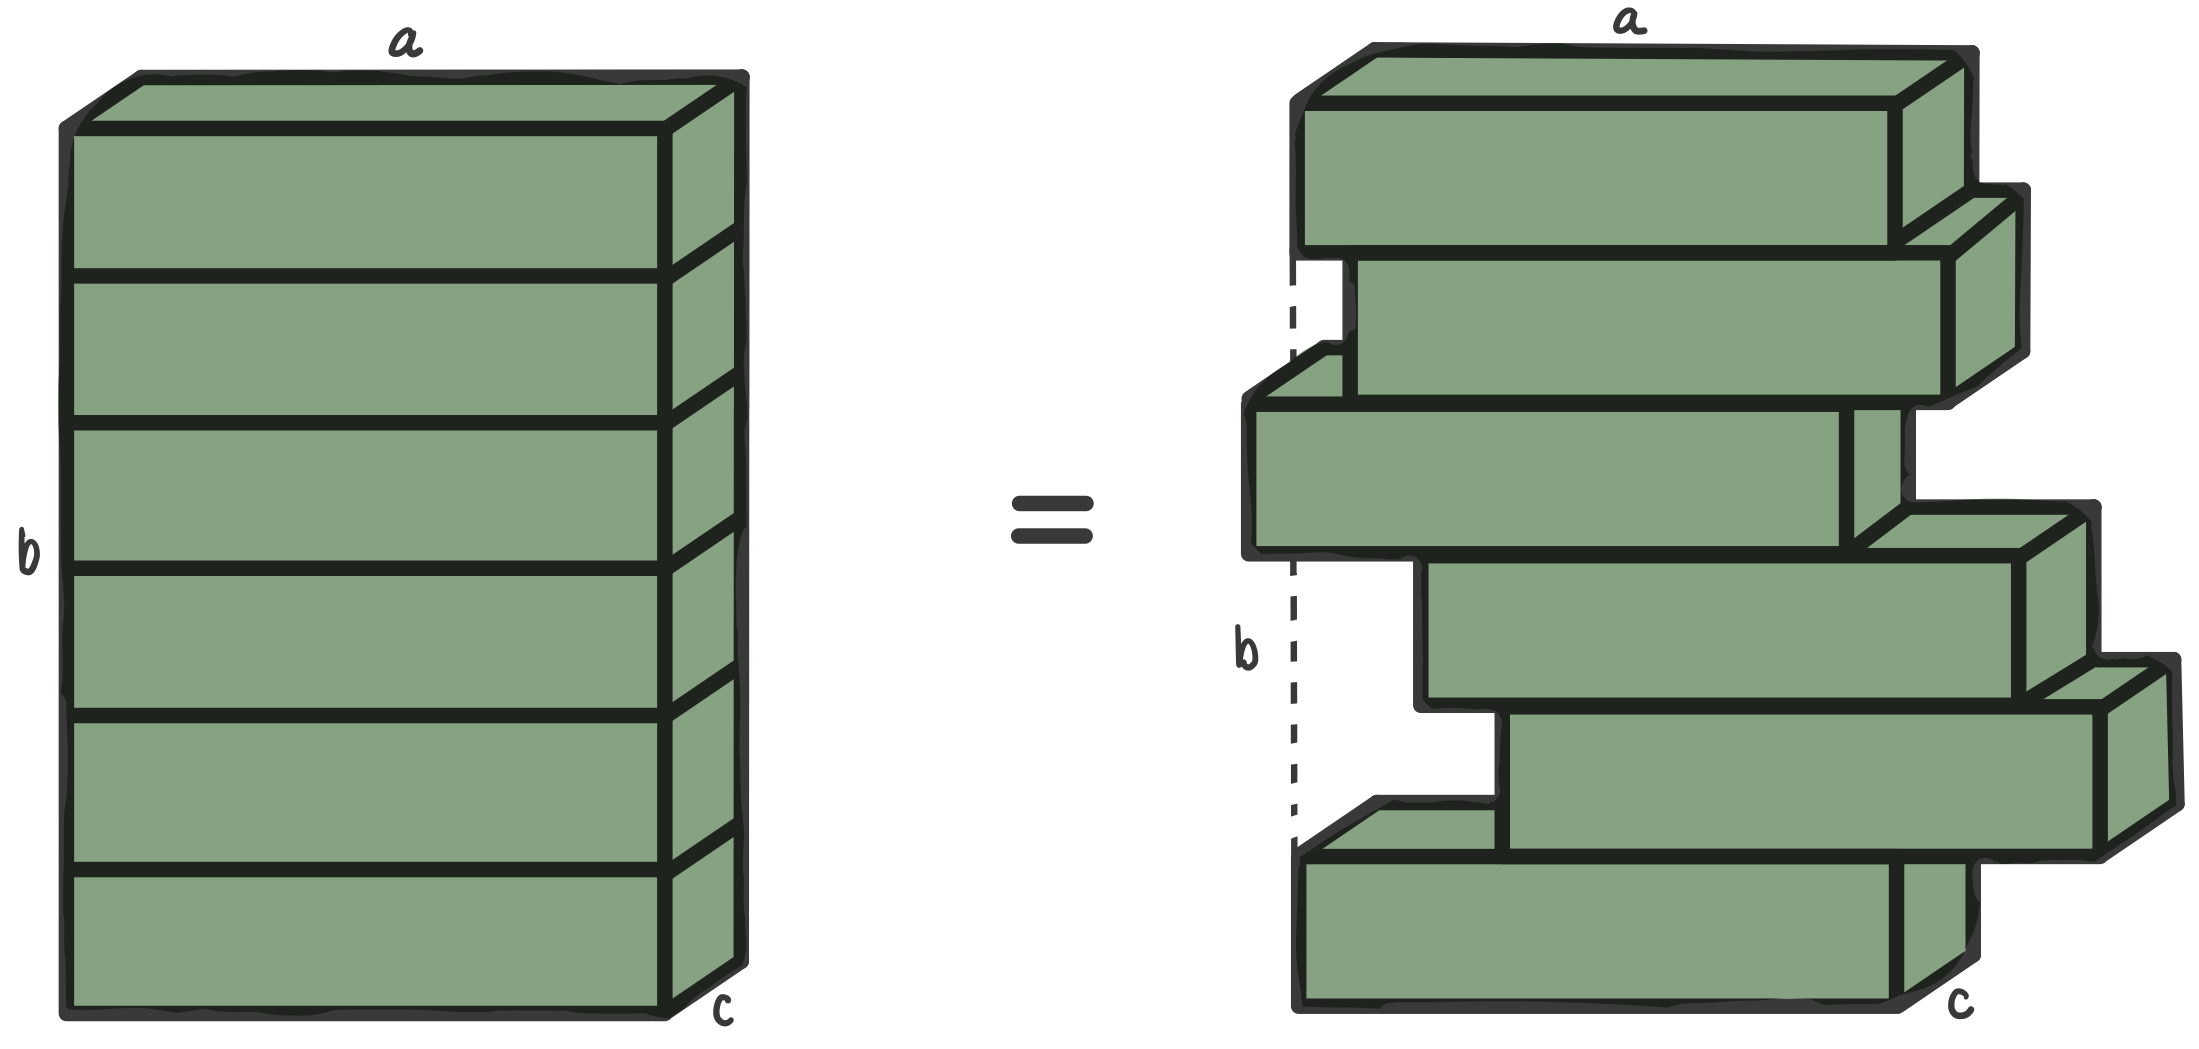
\includegraphics[width=\textwidth]{more images/cava1.jpg}
         \caption{Basis of Cavalieri's Principle}
         \label{fig:cavasimp}
     \end{subfigure}
     \hfill
     \begin{subfigure}[b]{0.45\textwidth}
         \centering
         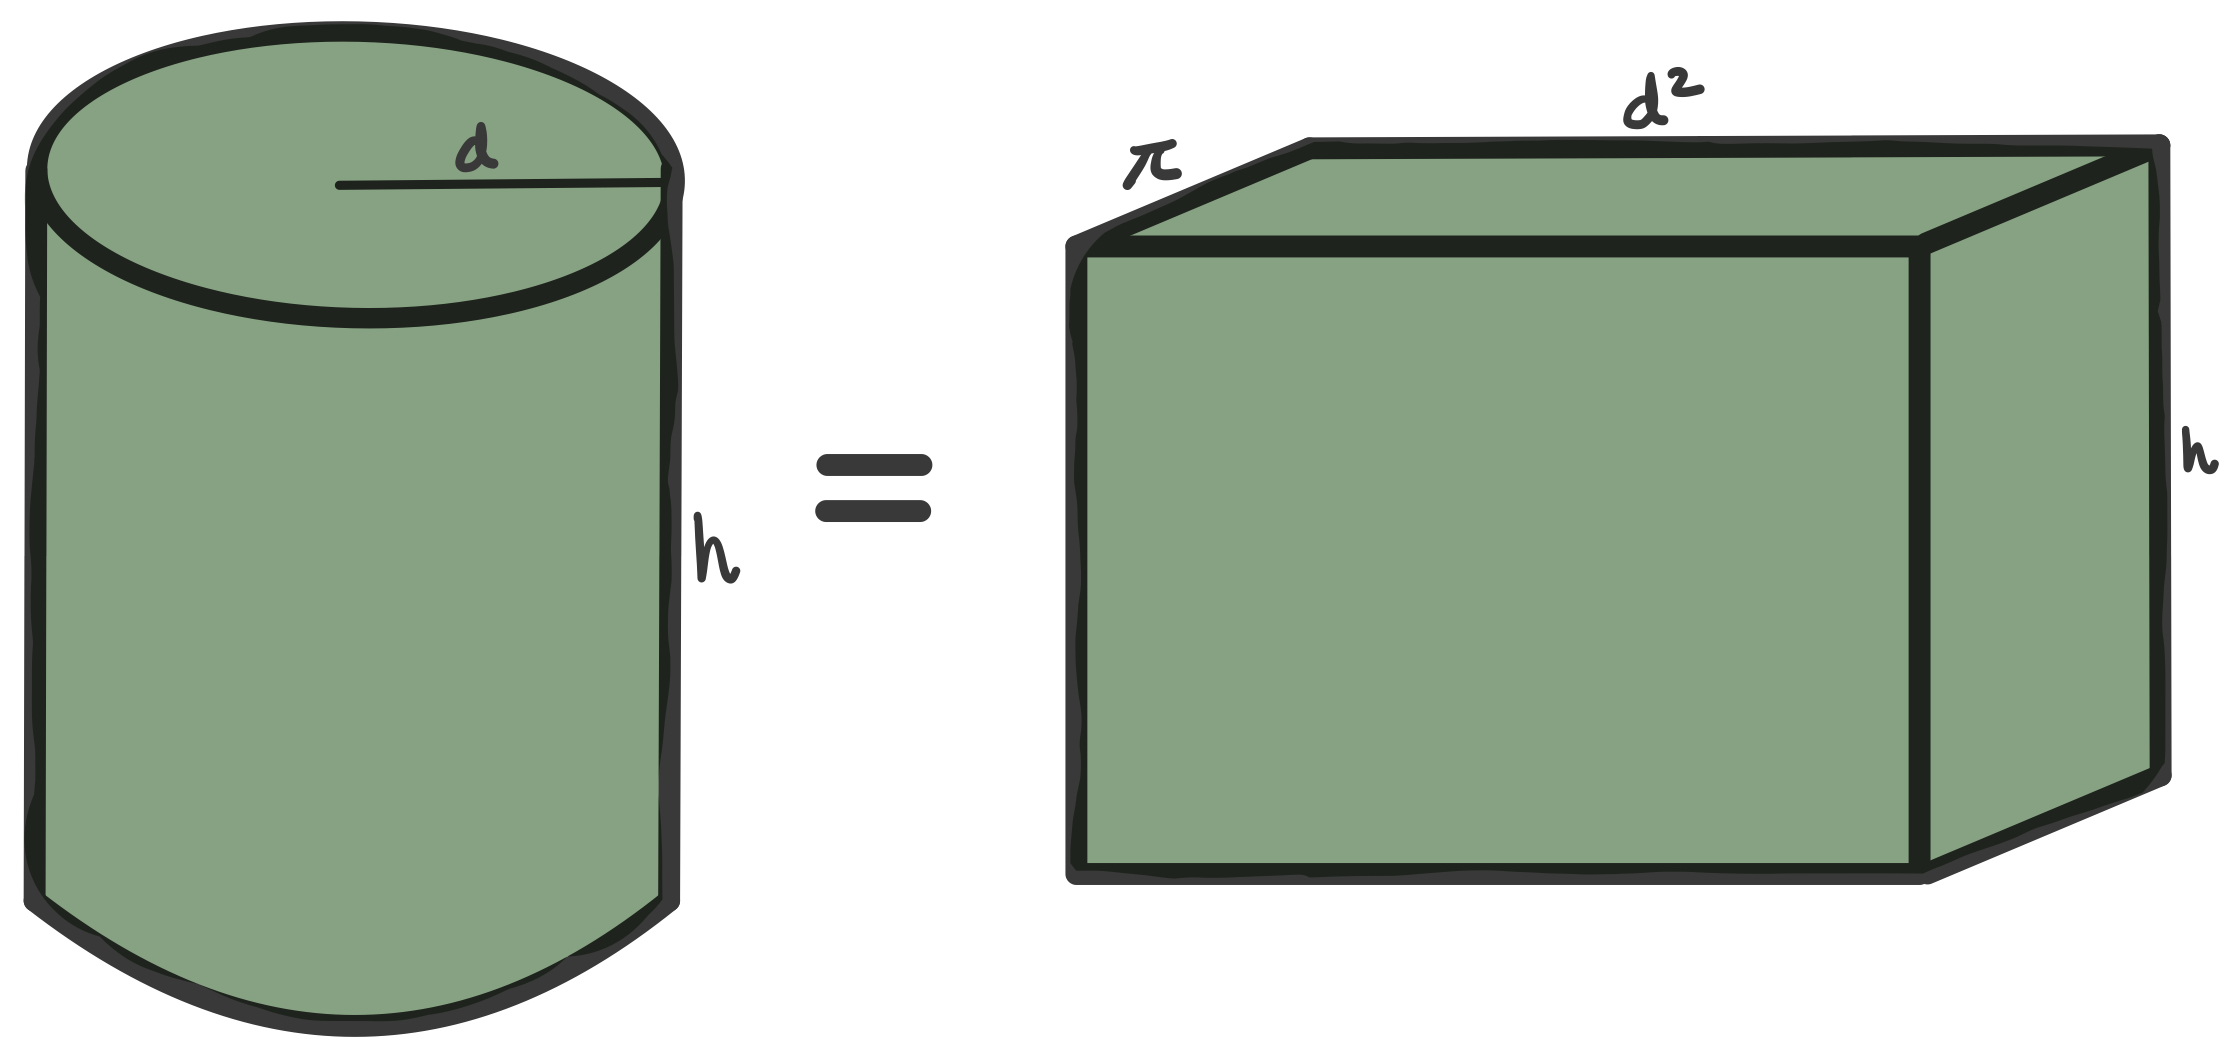
\includegraphics[width=\textwidth]{more images/cava2.jpg}
         \caption{Projecting onto a hypothetical shape}
         \label{fig:cavahypo}
     \end{subfigure}
     \hfill
        \caption{Visual representations of Cavalieri's Principle}
        \label{fig:cava}
\end{figure}

Hence, to carry out this investigation, we will find the volume of the teaspoon by using Cavalieri's Principle. Firstly, we will need to find the function for both the parabolas that model the curvature of the teaspoon. We can then create a hypothetical shape that shares the same cross sectional area as the elliptical paraboloid that models the spoons, but is simple to find the volume of. Finally, using this hypothetical shape as a reference, we can find an equation to solve for the volume of the elliptical paraboloid that the teaspoon is encapsulated by.

Through this method, we will be able to compare the results of the Cavalieri method to the volume measured by weight of my teaspoon, and evaluate the effectiveness of the Cavalieri method. We will also discover what the difference between my teaspoons and standard teaspoons is so I can know when cooking what the US standard measurements are equivalent to. 

\section{Modelling the Curves}

\subsection{The First Parabola}

Firstly, we need to measure the height, width and length of our teaspoon. The measurements taken with a ruler ($\pm 0.05$ cm) at the widest part are summarised below:

\begin{center}
    \begin{tabular}{@{} lr @{}}
        \toprule
            Teaspoon Measurements (cm)  \\
        \midrule
            Length & 4.15\\
            Width & 2.85\\
            Height & 0.80\\
        \bottomrule
    \end{tabular}
    \captionof{table}{Teaspoon measurement ($\pm 0.05$ cm)}
    \label{tab:measurements}
\end{center}

Now we need to determine the equations that model the curvature of the teaspoon. Using GeoGebra, we can import an image of the teaspoon from a side-view and front-view and scale it so the axes are equivalent to the actual measurements of the image of the spoon (Figure \ref{fig:scale}). Next, we can plot different points along the curve from each point of view (side and front) in order to develop a function (Figure \ref{fig:plot}). As any curve can be modelled by an infinitely high degree polynomial, we will use parabolas to model the curves for simplicity. To demonstrate, we can use the side view of the teaspoon as shown below in Figure \ref{fig:tsp geo1}:

\begin{figure}[h]
     \centering
     \begin{subfigure}[b]{0.45\textwidth}
         \centering
         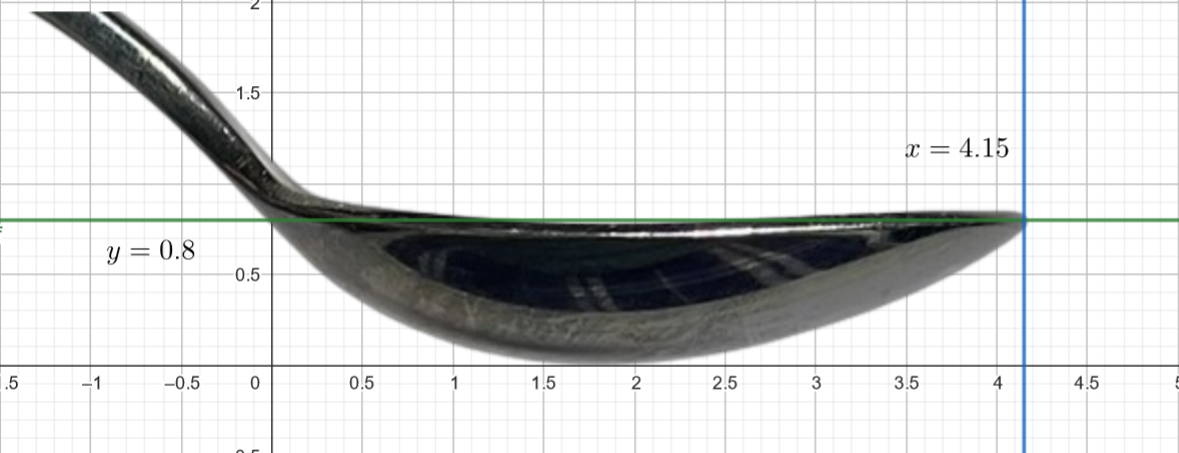
\includegraphics[width=\textwidth]{images/tsp bound.png}
         \caption{Scaling the teaspoon size to the axes}
         \label{fig:scale}
     \end{subfigure}
     \hfill
     \begin{subfigure}[b]{0.45\textwidth}
         \centering
         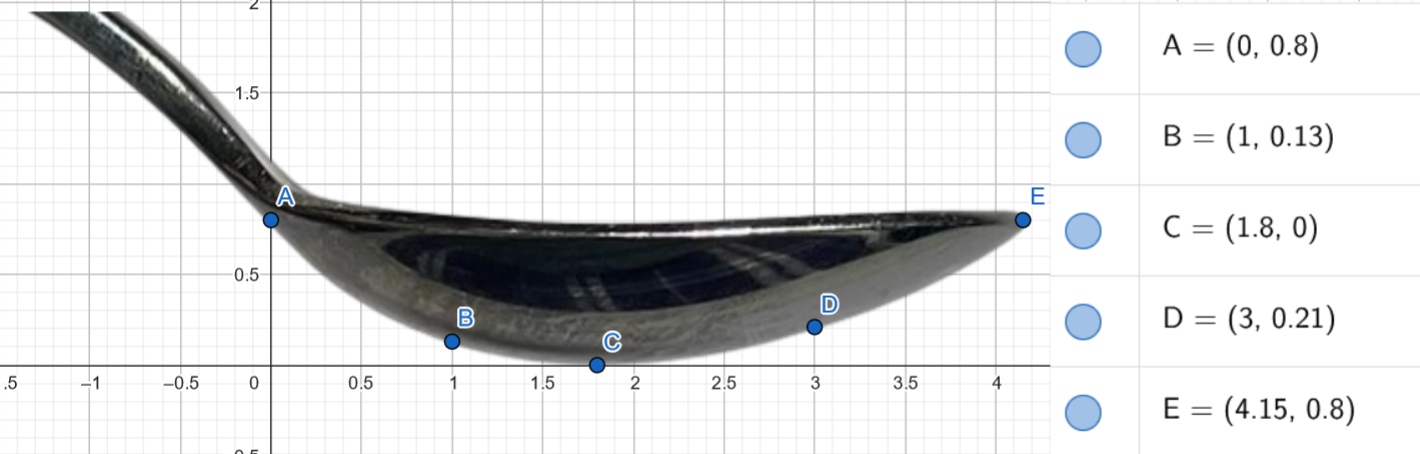
\includegraphics[width=\textwidth]{images/tsp with points.png}
         \caption{Plotting points along the curvature}
         \label{fig:plot}
     \end{subfigure}
     \hfill
        \caption{Using GeoGebra to model the equations}
        \label{fig:tsp geo1}
\end{figure}

As is evident by the difference in slope of each side of the teaspoon, the curvature is not a perfect parabola, but rather what appears to be a combination of two parabolas about the zero. Hence, we can create a piece-wise function utilising the plotted points to find the equations of both curves. 
Given that the points $A$, $B$, $C$, $D$ and $E$ (values indicated in Figure \ref{fig:plot}) are plotted along the curvature of the teaspoon side view, we can solve for the two parabolas which intersect at $x=1.8$. We will round all numbers to four decimal places throughout the investigation to maintain accuracy without compromising conciseness. \\

We can find the parabola of the teaspoon side-view, $f(x)=\alpha x^2+ \beta x+ \gamma$, over the domain $x \in [0,1.8]$ by solving for the variables $\alpha$, $\beta$, and $\gamma$ in $f(x)$ given that we know $A=(0,0.8)$, $B=(1,0.13)$ and $C=(1.8,0)$ through substitution and systems of equations demonstrated below:

$$
\begin{array}{l|c}
    y = \alpha x^2 + \beta x + \gamma & \text{Parabola } f(x) \\ \\
    (0.8) = \alpha (0)^2 + \beta (0) + \gamma & \text{Substitute } A=(0,0.8) \\ \\
 \end{array}
$$

\begin{equation}\label{solve.gamma}
    \boxed{\gamma = 0.8}  \quad \text{Solving for } \gamma
\end{equation}
 
$$
\begin{array}{l|c}
    y = \alpha x^2 + \beta x + \gamma & \text{Parabola } f(x) \\ \\
    (0.13) = \alpha (1)^2 + \beta (1) + \gamma & \text{Substitute } B=(1,0.13) \\ \\
    0.13 = \alpha + \beta + (0.8) & \text{Substituting } \gamma=0.8 \\ \\
 \end{array} 
$$

\begin{equation}\label{solve.alpha}
    \boxed{ \alpha = -0.67 - \beta }  \quad \text{Solving for } \alpha
\end{equation}

$$
\begin{array}{l|c}
    y = \alpha x^2 + \beta x + \gamma & \text{Parabola } f(x) \\ \\
    (0) = \alpha (1.8)^2 + \beta (1.8) + \gamma & \text{Substitute } C=(1.8,0) \\ \\
    0 = 3.24(-0.67 -\beta) + 1.8 \beta + (0.8) & \text{Substitute } \alpha =-0.67- \beta \text{ and } \gamma =0.8\\ \\
    1.44 \beta = -1.3708 & \text{Make } \beta \text{ the subject} \\ \\
\end{array}
$$

\begin{equation}\label{solve.beta}
    \boxed{ \beta = -0.9519}  \quad \text{Solving for } \beta
\end{equation}

$$
\begin{array}{l|c}
    \alpha = -0.67 - \beta & \text{Equation \ref{solve.alpha}}\\ \\
    \alpha = -0.67 -(-0.9519) & \text{Substitute } \beta =-0.9519 \\ \\
 \end{array} 
$$

\begin{equation}\label{solve.alpha2}
    \boxed{ \alpha = 0.2819}  \quad \text{Solving for } \alpha
\end{equation}

Now that we know the value of $\alpha$, $\beta$, and $\gamma$, we get the equation for the parabola modelling the left side of the teaspoon side-view:

\begin{equation}\label{f(x)}
    \boxed{f(x)=0.2819x^2 -0.9519x +0.8}
\end{equation}

The same method can be applied to find the second parabola for the right half of the teaspoon side view, $g(x)$, in the interval $x \in [1.8, 4.15]$, with the coordinates $C = (1.8,0)$, $D= (3,0.21)$ and $E=(4.15,0.8)$. Where $g(x)$ is the parabola $y=jx^2+kx+l$, we can substitute the $x$ and $y$ values of the coordinate points $C$, $D$, and $E$ to form a system of three equations with which we can solve for $j$, $k$, and $l$ as we did previously for $f(x)$ (Equation \ref{f(x)}). For conciseness, this process will not be shown as it is the same as Equations \ref{solve.gamma} to \ref{solve.alpha2}.

\vspace{-5mm}

\begin{equation}\label{g(x)}
    \boxed{g(x)= 0.1438x^2 -0.5155x + 0.4618}
\end{equation}

Thus we can construct the following piece-wise function (Equation \ref{h(x).pw}), where the functions switch at the zero, $x=1.8$, modelling the curvature of the side-view of the teaspoon also shown in Figure \ref{fig:tsp model}.

\begin{equation}\label{h(x).pw}
    h(x)=
    \begin{cases}
        0.2819x^2 - 0.9519x + 0.80 & \text{if } x \le 1.8 \\
        0.1438x^2 - 0.5155x + 0.4618 & \text{if } x \ge 1.8
    \end{cases}
\end{equation}

\begin{figure}[h]
    \centering
        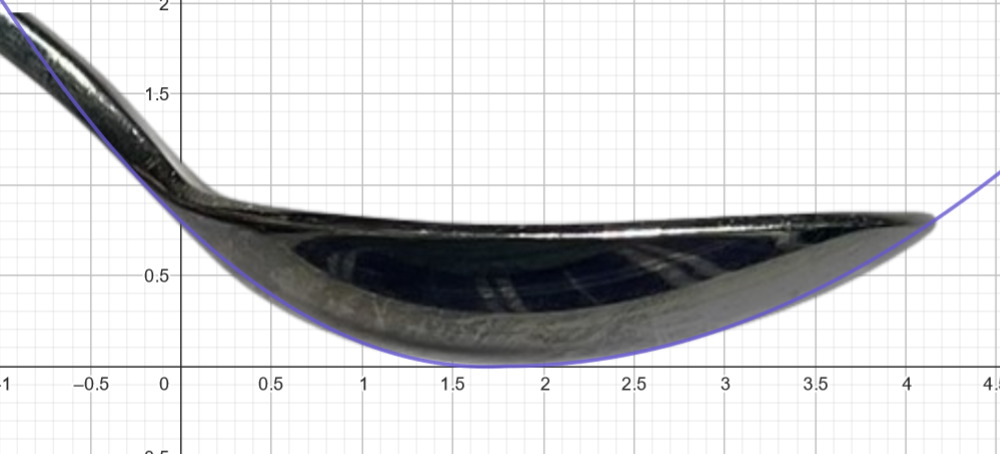
\includegraphics[scale=0.45]{images/modelled tsp.png}
        \caption{Piece-wise function, $h(x)$, plotted teaspoon image in GeoGebra}
    \label{fig:tsp model}
\end{figure}

However, we encounter a problem with the piece-wise function (\ref{h(x).pw}). If we wish to project an elliptical paraboloid onto a hypothetical shape through Cavalieri's Principle, the elliptical paraboloid must be in the terms of two parabolas and an ellipse - where this piece-wise function would be in lieu of one of the parabolas, complicating the projection.

Since there is an infinite combination of variables that can be used to form a volume, shown in my illustration, Figure \ref{fig:inf volumes}, then as long as the area encapsulated by any parabola is equivalent to that of the piece-wise function, $h(x)$, given the other parameters are the same, they should encapsulate the same volume. 

\begin{figure}[h]
    \centering
        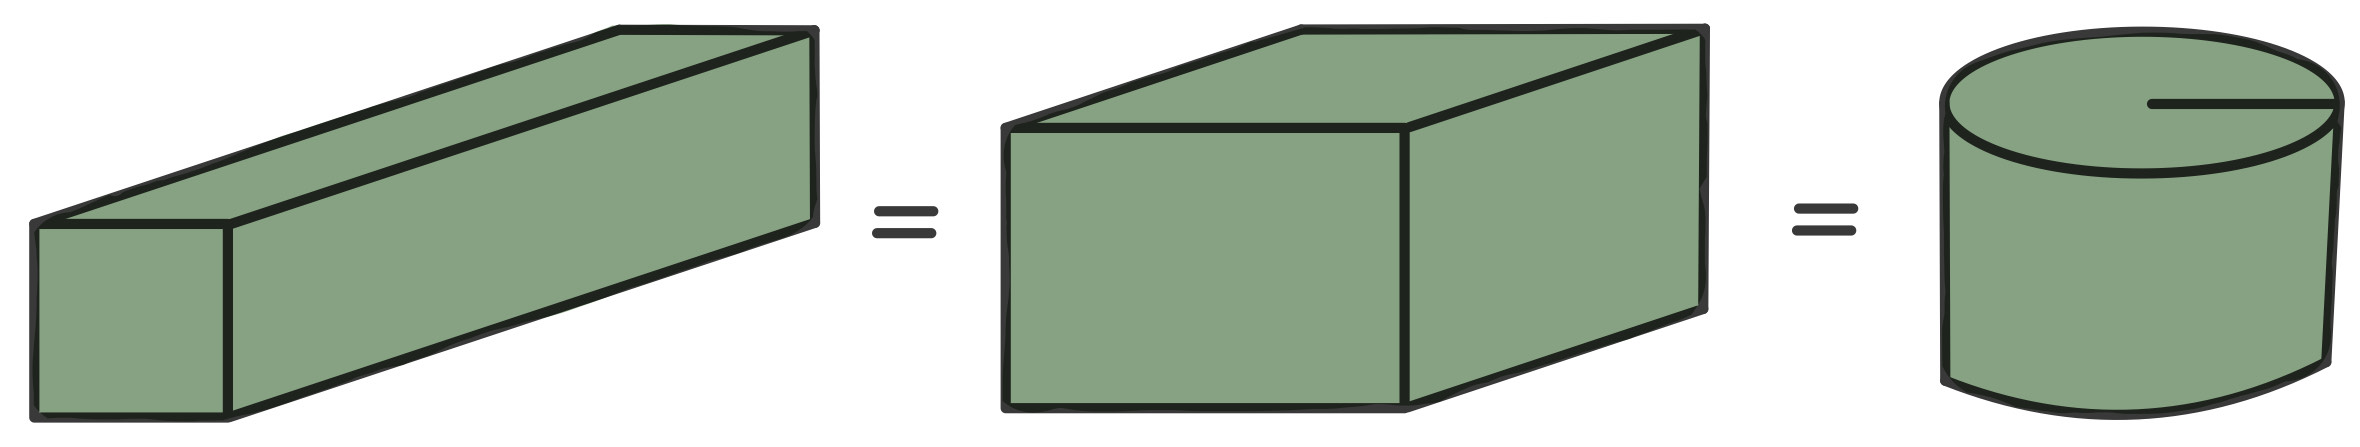
\includegraphics[scale=0.15]{images/volumes equiv.jpg}
        \caption{Hypothetical solids of equal volumes have infinite possibilities to encapsulate one volume}
    \label{fig:inf volumes}
\end{figure}

Using this reasoning, I initially thought to take the average of the two parabolas ($f(x)$ and $g(x)$) within the piece-wise function $h(x)$. However, after modelling this situation on GeoGebra (Figure \ref{fig:avg problem}), I quickly realised my error - $h(x)$ does not switch between the parabolas at the domain midpoint of the teaspoon side-view, but rather the point at which both parabolas are at zero. This caused the problem that was highlighted when using the GeoGebra integral between function for $h(x)$ and the proposed average function of $f(x)$ and $g(x)$ (Figure \ref{fig:skill-issue}). The two areas were not equivalent because average takes the midpoint of two values but these two functions were not separated at the midpoint. 

\begin{figure}[h]
     \centering
     \begin{subfigure}[b]{0.45\textwidth}
         \centering
         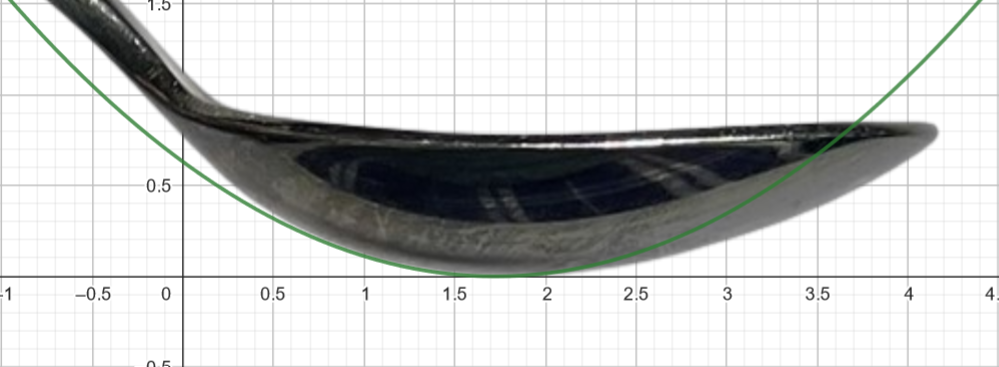
\includegraphics[width=\textwidth]{images/avg parab.png}
         \caption{Graphing the average of $f(x)$ and $g(x)$}
         \label{fig:avg.parab}
     \end{subfigure}
     \hfill
     \begin{subfigure}[b]{0.45\textwidth}
         \centering
         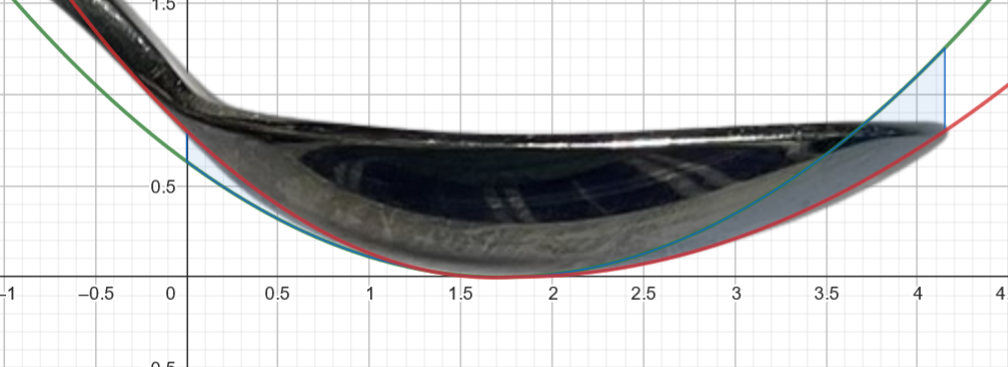
\includegraphics[width=\textwidth]{images/uneq area.png}
         \caption{Integral between both functions}
         \label{fig:skill-issue}
     \end{subfigure}
     \hfill
        \caption{Using GeoGebra to model the average function of $f(x)$ and $g(x)$}
        \label{fig:avg problem}
\end{figure}

\pagebreak

I still liked this approach to simplifying the piece-wise function, $h(x)$, into a parabola so I continued along that path. Let us call this hypothetical parabola that simplifies the piece-wise function $p(x)$. $p(x)$ would be a parabola in which the area between itself and the piece-wise function on the left half is equivalent to that on the right. That is to say, any area that is added under the teaspoon side-view from the one side is then cancelled by the area that is subtracted from the teaspoon side view on the other (attempted in \ref{fig:skill-issue}) in a sort of visually intuitive way that changes the shape of the teaspoon slightly without actually compromising the volume calculated as discussed in Figure \ref{fig:inf volumes}.

With this hypothetical parabola, $p(x)$, and using the halves of our piece-wise function $h(x)$ individually, ($f(x)$ and $g(x)$), we can say the following:

$$
\begin{array}{l|c}
    \int_0^{1.8}{(f(x)-p(x))}dx = \int_{1.8}^{4.15}{(p(x)-g(x))}dx & \text{Finding area bound} \\ \\
    \int_0^{1.8}{f(x)}dx - \int_0^{1.8}{p(x)}dx = \int_{1.8}^{4.15}{p(x)}dx - \int_{1.8}^{4.15}{g(x)}dx & \text{Distributing integral} \\ \\
    \int_0^{1.8}{p(x)}dx + \int_{1.8}^{4.15}{p(x)}dx = \int_0^{1.8}{f(x)}dx +\int_{1.8}^{4.15}{g(x)}dx & \text{Making } p(x) \text{ the subject}\\ \\
 \end{array}
$$

\vspace{-8mm}

\begin{equation}\label{tsp def ints}
    \boxed{\int_{0}^{4.15}{p(x)}dx = \int_0^{1.8}{f(x)}dx +\int_{1.8}^{4.15}{g(x)}dx}  \quad \text{Summing the limits of the integral}
\end{equation}

The conclusion in Equation \ref{tsp def ints} that the area under the curve of our hypothetical parabola $p(x)$ in the interval $x \in [0,4.15]$ is equivalent to the sum of the areas under the curves $f(x)$, $x \in [0,1.8]$, and $g(x)$, $x \in [1.8,4.15]$, is intuitive. 

Let $p(x)$ be the parabola $y=qx^2$. This parabola can be modelled with just an $x^2$ variable because of the idea explored in Figure \ref{fig:inf volumes}. Regardless of the \textit{shape} of a solid, it can still hold an equivalent volume to another solid given certain dimensions, as there are infinite possibilities to model a single volume. We can recognise that the shape of the teaspoon will be more deformed by only having one variable in this parabola, however, this simplifies the problem while maintaining the areas, and thus volumes, equivalent. 

Since we know both $f(x)$ and $g(x)$ and now we have $p(x)=qx^2$, we can solve for the parabola $p(x)$ needed to calculate the volume of the teaspoon through Cavalieri's Principle using the definite integrals from Equation \ref{tsp def ints} demonstrated below:

$$
\begin{array}{l|c}
    \int_0^{1.8}{f(x)}dx = \int_0^{1.8}{(0.2819x^2 -0.9519x +0.8)}dx & \text{Substituting } f(x) \\ \\
    = \left[   \frac{0.2819}{3}x^3 -  \frac{0.9519}{2}x^2 + 0.80x \right]_0^{1.8} & \text{Solving integral} \\ \\
    = (\frac{0.2819}{3}(1.8)^3 - \frac{0.9519}{2}(1.8)^2 + 0.80(1.8)) & \text{Substituting } x=1.8 \\
    \quad -(\frac{0.2819}{3}(0)^3 - \frac{0.9519}{2}(0)^2 + 0.80(0))  & \text{and } x=0 \\ \\
    \int_0^{1.8}{f(x)}dx = 0.5480 - 1.5421 + 1.44 -0 & \text{Simplifying} \\ \\
 \end{array}
$$

\begin{equation}\label{tsp.int.fx}
    \boxed{\int_0^{1.8}{f(x)}dx = 0.4459}  \quad \text{Arriving at}
\end{equation}

$$
\begin{array}{l|c}
   \int_{1.8}^{4.15}{g(x)}dx = \int_{1.8}^{4.15}{(0.1438x^2 -0.5155x + 0.4618)}dx & \text{Substituting g(x)} \\ \\
    = \left[   \frac{0.1438}{3}x^3 -  \frac{0.5155}{2}x^2 + 0.4618x \right]_{1.8}^{4.15} & \text{Solving integral} \\ \\
    = (\frac{0.1438}{3}(4.15)^3 - \frac{0.5155}{2}(4.15)^2 + 0.4618(4.15)) & \text{Substituting } x=4.15 \\ \quad -(\frac{0.1438}{3}(1.8)^3 - \frac{0.5155}{2}(1.8)^2 + 0.4618(1.8)) & \text{and } x=1.8 \\ \\
\end{array}
$$

$$
\begin{array}{l|c}
    \int_{1.8}^{4.15}{g(x)}dx = 0.9033 -0.2757 & \text{Simplifying} \\ \\
 \end{array}
$$

\begin{equation}\label{tsp.int.gx}
    \boxed{\int_{1.8}^{4.15}{g(x)}dx = 0.6277}  \quad \text{Arriving at}
\end{equation}

$$
\begin{array}{l|c}
   \int_{0}^{4.15}{p(x)}dx = \int_{0}^{4.15}{px^2}dx & \text{Substituting p(x)} \\ \\
    = \left[   \frac{p}{3}x^3   \right]_0^{4.15} & \text{Solving integral} \\ \\
    = (\frac{p}{3}(4.15)^3) - (\frac{p}{3}(0)^3) & \text{Substituting } x=4.15 \text{ and } x=0 \\ \\
    \int_{0}^{4.15}{p(x)}dx = \frac{4.15^3}{3}p & \text{Simplifying} \\ \\
 \end{array}
$$

\begin{equation}\label{tsp.int.px}
    \boxed{\int_{0}^{4.15}{p(x)}dx = 23.8245p}  \quad \text{Arriving at}
\end{equation}

Now, we can solve Equation \ref{tsp def ints} by substituting back the values obtained in equations \ref{tsp.int.fx}, \ref{tsp.int.gx}, and \ref{tsp.int.px}, allowing us to find the value $p$, and hence, solve for the parabola $p(x)$.

$$
\begin{array}{l|c}
    \int_{0}^{4.15}{p(x)}dx = (0.4459) +(0.6277) & \text{Substituting } f(x) \text{ and } g(x) \\ \\
    23.8245p = 1.0736 & \text{Substituting } \int_{0}^{4.15}{p(x)}dx \\ \\
 \end{array}
$$

\begin{equation}\label{tsp.int}
    \boxed{p = 0.0451}  \quad \text{Solving for } p
\end{equation}

Hence, our parabola with an area equivalent to our piece-wise function, $h(x)$, is $p(x)=0.0451x^2$. We can check this by graphing both equations and comparing the integrals on GeoGebra as shown in Figure \ref{fig:ints.geo}.

\vspace{-8mm}

\begin{equation}\label{p(x)}
    \boxed{p(x)=0.0451x^2}
\end{equation}

\begin{figure}[h]
     \centering
     \begin{subfigure}[b]{0.4\textwidth}
         \centering
         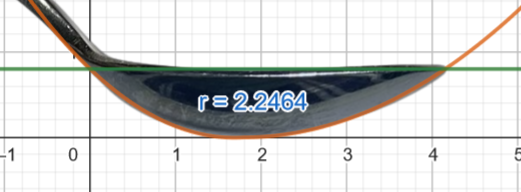
\includegraphics[width=\textwidth]{more images/intbw r.png}
         \caption{Integral bound by $y=0.8$ and $h(x)$}
         \label{fig:pwabove}
     \end{subfigure}
     \hfill
     \begin{subfigure}[b]{0.4\textwidth}
         \centering
         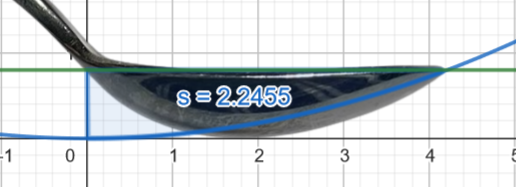
\includegraphics[width=\textwidth]{more images/int btw s.png}
         \caption{Integral bound by $y=0.8$ and $p(x)$}
         \label{fig:pxabove}
     \end{subfigure}
     \hfill
\end{figure}

Figure \ref{fig:pwabove} shows the area of the teaspoon side-view, $r$, represented by the integral bound between the line $y=0.8$ (the height of the spoon) and the piece-wise function $h(x)$. From the GeoGebra graphing tools, we can see that $r=2.2464$. Similarly, $p(x)$ in Figure \ref{fig:pxabove} shows a very different looking shape but with the area $s$. For $p(x)$, $s=2.2455$, showing that $s$ is approximately equal to $r$, supporting the conclusion that within the interval of $x \in [0,4.15]$, the functions $p(x)$ and $h(x)$ have the same area. 

The slight differences in calculations are most likely due to error introduced when rounding, but when considering four significant figures, this error is eliminated. Although it is almost insignificant, it still is important to note that the area in the interval $x \in [0,4.15]$ for $p(x)$ is not exactly equal to that of $h(x)$. As these functions are transformed further throughout this investigation, this error may become more significant. 

\subsection{The Second Parabola}
We can now start to repeat the process we used to find the first parabola, $p(x)$, to find the other parabola that encapsulates the front-view of the teaspoon. I found modelling the spoon with a photo import on GeoGebra to be very efficient and visually intuitive, hence I will use the same process.

We can start by scaling the spoon image where $1$ cm $=1$ unit by graphing the lines $y=0.8$ and $x=2.85$ as reference boundaries, since the height and width of the spoon are 0.8 cm and 2.85 cm respectively (Table \ref{tab:measurements}). Since the front-view of the teaspoon is symmetrical, we will only need one parabola to model it. Let us call this parabola $o(x)$ in which $y=tx^2 + ux +v$ (noting that $t$ is different from $T$ and so on). As we will be using the same method as in Equations \ref{solve.gamma} to \ref{f(x)} to solve for $o(x)$, the intermediate steps will not be shown for conciseness.  

\pagebreak

\begin{figure}[h]
     \centering
     \begin{subfigure}[b]{0.45\textwidth}
         \centering
         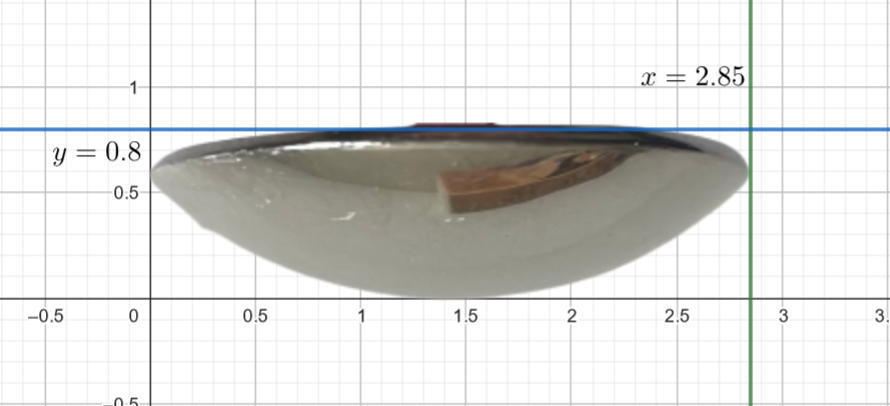
\includegraphics[width=\textwidth]{images/tsp scale.png}
         \caption{Scaling the teaspoon size to the axes}
         \label{fig:scale}
     \end{subfigure}
     \hfill
     \begin{subfigure}[b]{0.45\textwidth}
         \centering
         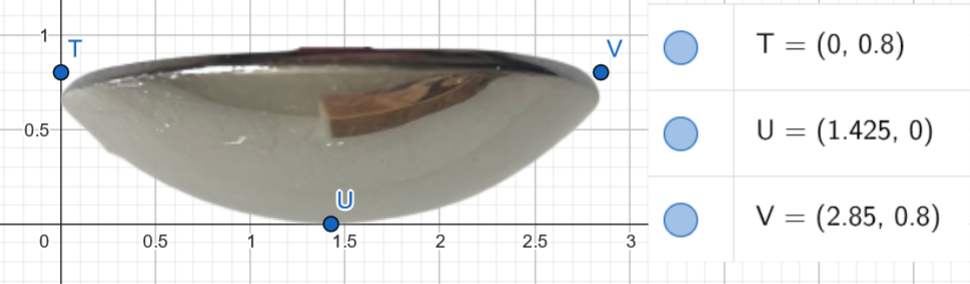
\includegraphics[width=\textwidth]{images/tsp points.png}
         \caption{Plotting points along the curvature}
         \label{fig:plot}
     \end{subfigure}
     \hfill
        \caption{Using GeoGebra to model the teaspoon front-view}
        \label{fig:tsp geo2}
\end{figure}

Given the coordinates $T=(0,0.8)$, $U=(1.425,0)$, and $V=(2.85,0.8)$, let us solve for $o(x)=tx^2+ux+v$ by creating a system of three equations and using substitution:

\begin{equation}\label{solve.v}
    \boxed{v = 0.8}  \quad \text{Solving for } v
\end{equation}

\begin{equation}\label{solve.u}
    \boxed{u = -1.425t -0.5614}  \quad \text{Solving for } u
\end{equation}

\begin{equation}\label{solve.t}
    \boxed{t = 0.3940}  \quad \text{Solving for } t
\end{equation}

\begin{equation}\label{solve.u2}
    \boxed{u = -1.1228}  \quad \text{Solving for } u
\end{equation}

As we know $t$, $u$, and $v$, we can get the equation for the parabola modelling the front-view of the teaspoon and graph it as well (Figure \ref{fig:fv tsp model}):

\begin{equation}\label{o(x)}
    \boxed{o(x)= 0.3940x^2 -1.1228 x +0.8}
\end{equation}

\begin{figure}[h]
    \centering
        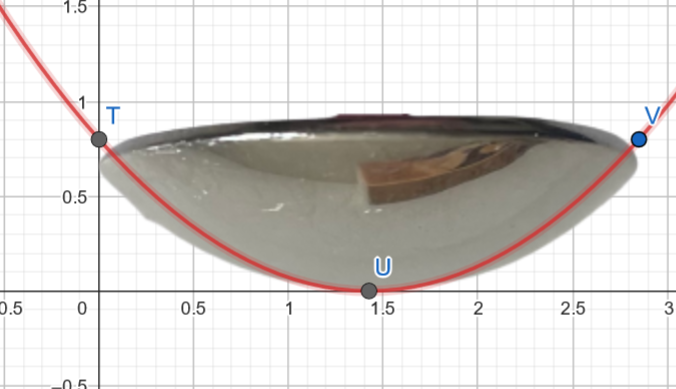
\includegraphics[scale=0.45]{images/fv.tspcurve.png}
        \caption{Parabola, $o(x)$, plotted over image of the teaspoon front-view in GeoGebra}
    \label{fig:fv tsp model}
\end{figure}

\pagebreak

It appears that the graph of $o(x)$ appears does not model the parabola very well. However, I chose to model the parabola based on the points $T$, $U$, and $V$ as the position of these coordinates is relative to the actual height and width of the parabola. The photo of the teaspoon from a front view is taken from a strange angle (albeit the best angle I could), and is slightly warped to fit the axes. As a result, I opted to place my reference coordinates $T$, $U$, and $V$ on known positions of the parabola, with the zero $U$ at the line of symmetry, and both $T$ and $V$ at the extremes of the height and width intersections, rather than base the coordinates on a warped image. Thus we can assume the equation $o(x)$ accurately models the front-view of the teaspoon.

While Equation \ref{o(x)}, $o(x)$ is useful, it is a bit complicated to use as it varies with $x^2$ and $x$. By the same principles and method we used when finding Equation \ref{p(x)}, $p(x)$, that an area can be modelled by infinitely many shapes given certain dimensions, we can find another parabola, $w(x)$, that has the same area over the domain $x \in [0,2.85]$ but is in simpler terms of just $x^2$. 

As we determined previously, if the integral of our proposed function $w(x)$ is equal to that of $o(x)$, then the areas bound by our parabolas and the height, $y=0.8$, will be equal. Since we know the equation for $o(x)$ we can say the following:

$$
\begin{array}{l|c}
    \int_0^{2.85}{w(x)}dx = \int_{0}^{2.85}{o(x)}dx & \text{Integral equivalency} \\ \\
    = \int_{0}^{2.85}{(0.3940x^2 -1.1228 x +0.8)}dx & \text{Substituting } o(x) \\ \\
    = \left[   \frac{0.3940}{3}x^3 \frac{-1.1228}{2}x^2 + 0.8x \right]_0^{2.85} & \text{Solving integral} \\ \\
    = (0.1313(2.85)^3 -0.5614(2.85)^2 + 0.8(2.85)) & \text{Substituting } x=2.85 \\ 
    \quad - (0.1313(0)^3 -0.5614(0)^2 + 0.8(0)) & \text{ and } x=0 \\ \\
    \int_0^{2.85}{w(x)}dx = 3.0395 -4.5600 +2.28 & \text{Simplifying}
 \end{array}
$$

\begin{equation}\label{int.wx}
    \boxed{\int_0^{2.85}{w(x)}dx = 0.7595}  \quad \text{Arriving at}
\end{equation}

Since we know $w(x)$ is a parabola is the form $y=ix^2$ (note that $i \in \mathbb{R}$), we can then solve for the integral in Equation \ref{int.wx}.

$$
\begin{array}{l|c}
    \int_0^{2.85}{w(x)}dx = \int_0^{2.85}{(ix^2)}dx & \text{Substituting } w(x) \\ \\
    = \left[   \frac{i}{3}x^3   \right]_0^{2.85} & \text{Solving integral} \\ \\
    = (\frac{i}{3}(2.85)^3) - (\frac{i}{3}(0)^3) & \text{Substituting } x=2.85 \text{ and } x=0 \\ \\
    \int_0^{2.85}{w(x)}dx = \frac{2.85^3}{3}i & \text{Simplifying} \\ \\
 \end{array}
$$

\begin{equation}\label{solve.i}
    \boxed{\int_0^{2.85}{w(x)}dx = 7.7164i}  \quad \text{Arriving at}
\end{equation}

Now we can solve for $i$ and the parabola $w(x)$ as we can equate Equations \ref{int.wx} and \ref{solve.i}:

$$
\begin{array}{l|c}
    0.7595 = 7.7164i & \text{Equating Equations \ref{int.wx} and \ref{solve.i}} \\ \\
    i = 0.0984 & \text{Simplifying} \\ \\
 \end{array}
$$

\begin{equation}\label{solve.i2}
    \boxed{i = 0.0984}  \quad \text{Arriving at}
\end{equation}

Thus, we have found the equation for our second parabola, $w(x)$, that models our teaspoon (Equation \ref{w(x)}). We can also graphically model this in GeoGebra confirming that both the integrals bound by the height $y=0.8$ and the respective parabola are equal as shown in Figure \ref{fig:para2.graph}.

\vspace{-8mm}

\begin{equation}\label{w(x)}
    \boxed{w(x) = 0.0984x^2}
\end{equation}

\begin{figure}[h]
     \centering
     \begin{subfigure}[b]{0.45\textwidth}
         \centering
         \includegraphics[width=\textwidth]{more images/mu friction?!.png}
         \caption{Integral bound by $y=0.8$ and $o(x)$}
         \label{fig:ox.graph}
     \end{subfigure}
     \hfill
     \begin{subfigure}[b]{0.45\textwidth}
         \centering
         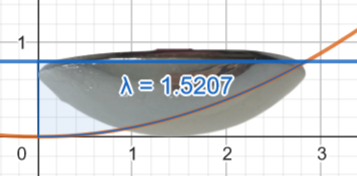
\includegraphics[width=\textwidth]{more images/lambda babay.png}
         \caption{Integral bound by $y=0.8$ and $w(x)$}
         \label{fig:wx.graph}
     \end{subfigure}
     \hfill
        \caption{Comparing the integrals of $o(x)$ and $w(x)$}
        \label{fig:para2.graph}
\end{figure}

Figures \ref{fig:ox.graph} and \ref{fig:wx.graph} show how these graphs of different parabolas have the same area over the domain $x \in [0,2.85]$ when bound by the line $y=0.8$. We can see that these areas are not exactly equal. Letting $\mu$ equal the area of $o(x)$, and $\lambda$ equal the area of $w(x)$ both bound by the curve $y=0.8$ we can see how the area of $o(x)$ is $\mu = 1.5197$, while the area of $w(x)$ is $\lambda = 1.5207$. To three significant figures these areas are equivalent, however, the fact that they are not introduces further error continuing forward in the investigation.

\section{Cavalieri's Principle}

Now that we've mathematically modelled the teaspoon in two-dimensions, we can combine these two parabolas to form a three dimensional shape (an elliptical paraboloid), and then transform it from a complex three dimensional solid, to a simpler three dimensional solid by applying Cavalieri's Principle as explained in Section \ref{method}. 

\begin{figure}[h]
    \centering
        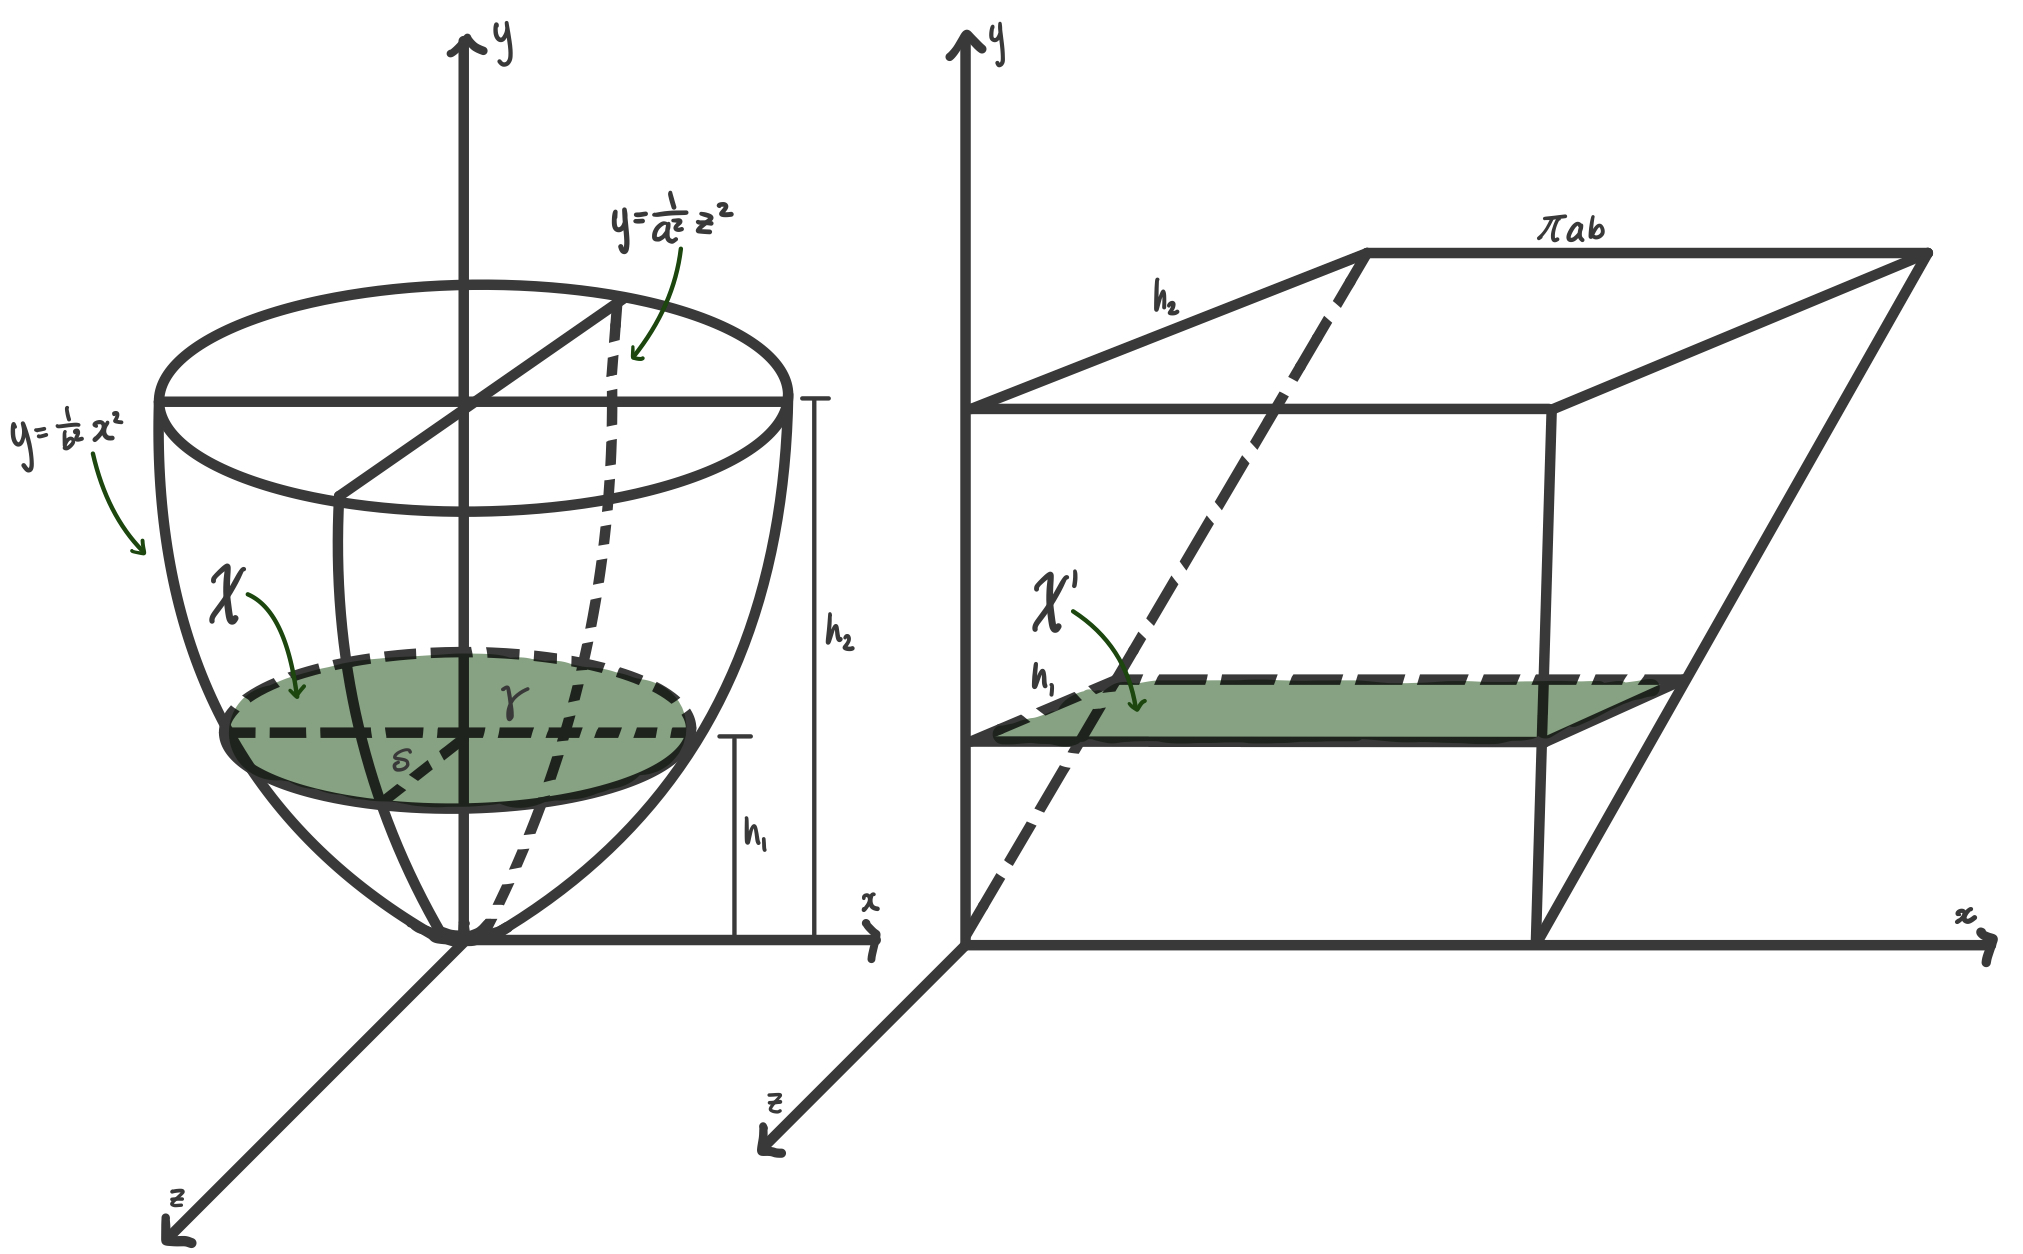
\includegraphics[width=0.6\textwidth]{more images/cava baby.jpg}
        \caption{Projecting the elliptical paraboloid onto a triangular prism}
        \label{fig:cava}
    \hfill
\end{figure}

The basis of this transformation will be taking our elliptical paraboloid, and transforming it into a triangular prism (\citeauthor{bogomolny}). I have drawn the transformation in Figure \ref{fig:cava} above, where the cross sectional area of the elliptical paraboloid, $\chi$, is equal to the of the triangular prism, $\chi '$.

To understand how this transformation works, we will dissect each component individually. We can start with the lengths $\gamma$ and $\delta$ on the cross section $\chi$. These are the semi-major and semi-minor axes of the ellipse, respectively. If we look at the parabola $y=\frac{1}{b^2}x^2$ on the 2-D plane $x$-$y$ (Figure \ref{fig:xy}), we can note that the length of $\gamma$ is actually a length along the $x$-axis as the cross-section $\chi$ is parallel to the $x$-axis. We can also note that the height, $h$ (noting that $h$ is different from $h(x)$ earlier in the investigation) is parallel to the $y$-axis, hence it is a length along the $y$-axis. 

\begin{figure}[h]
     \centering
     \begin{subfigure}[b]{0.45\textwidth}
         \centering
         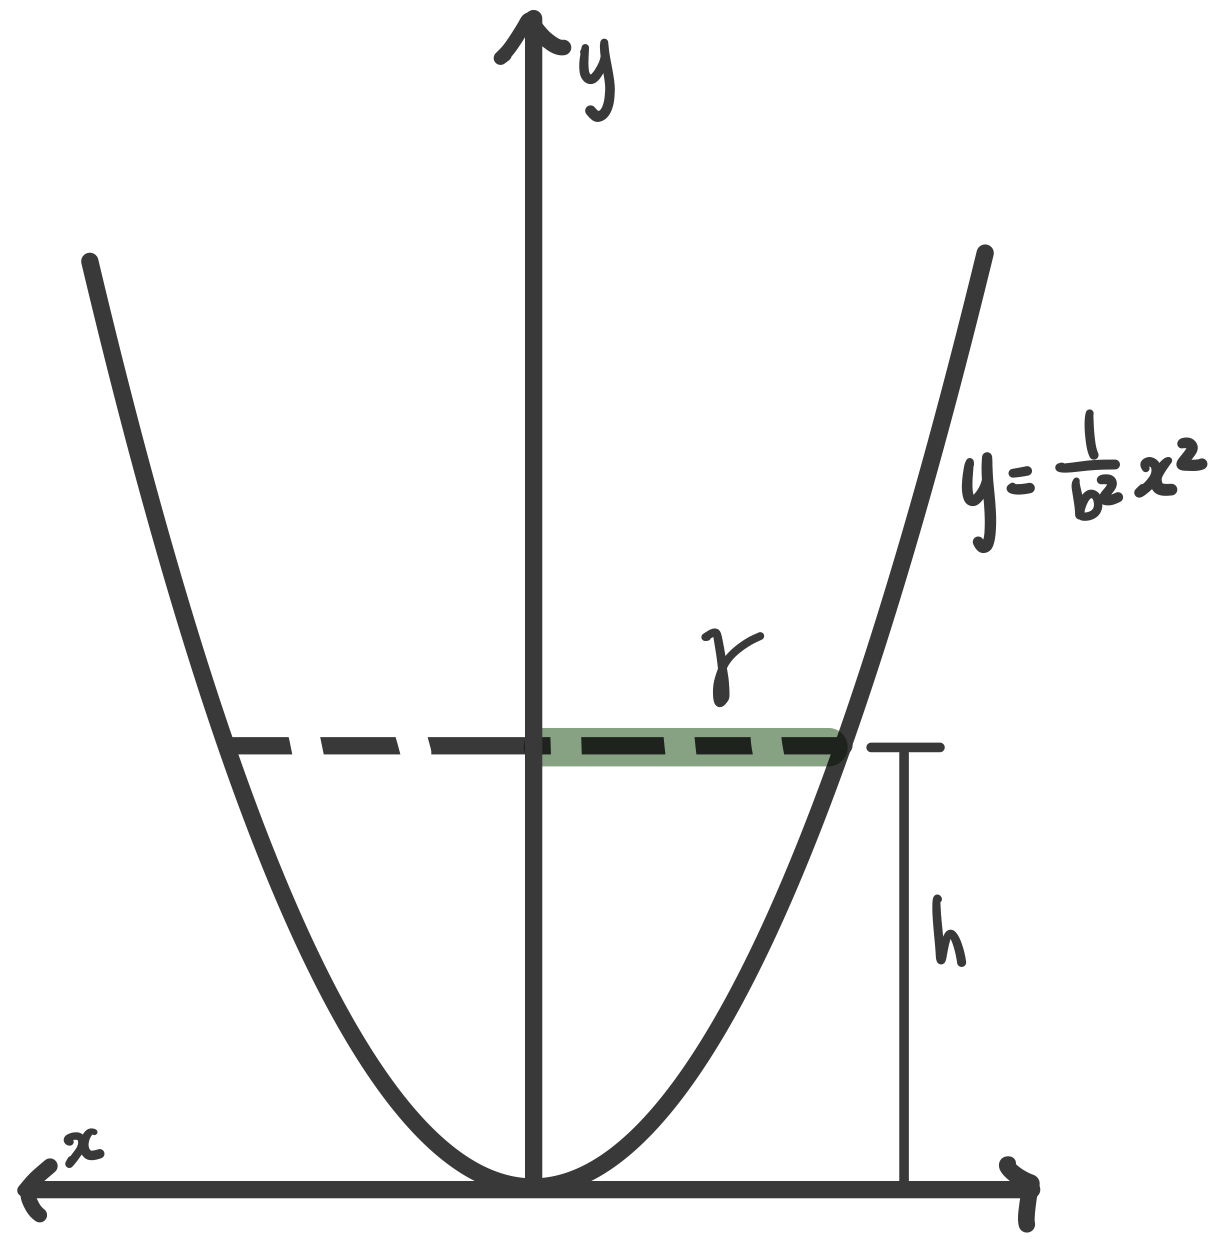
\includegraphics[width=0.6\textwidth]{more images/gamma.jpg}
         \caption{Major semi-axis length on $x$-$y$ plane}
         \label{fig:xy}
     \end{subfigure}
     \hfill
     \begin{subfigure}[b]{0.45\textwidth}
         \centering
         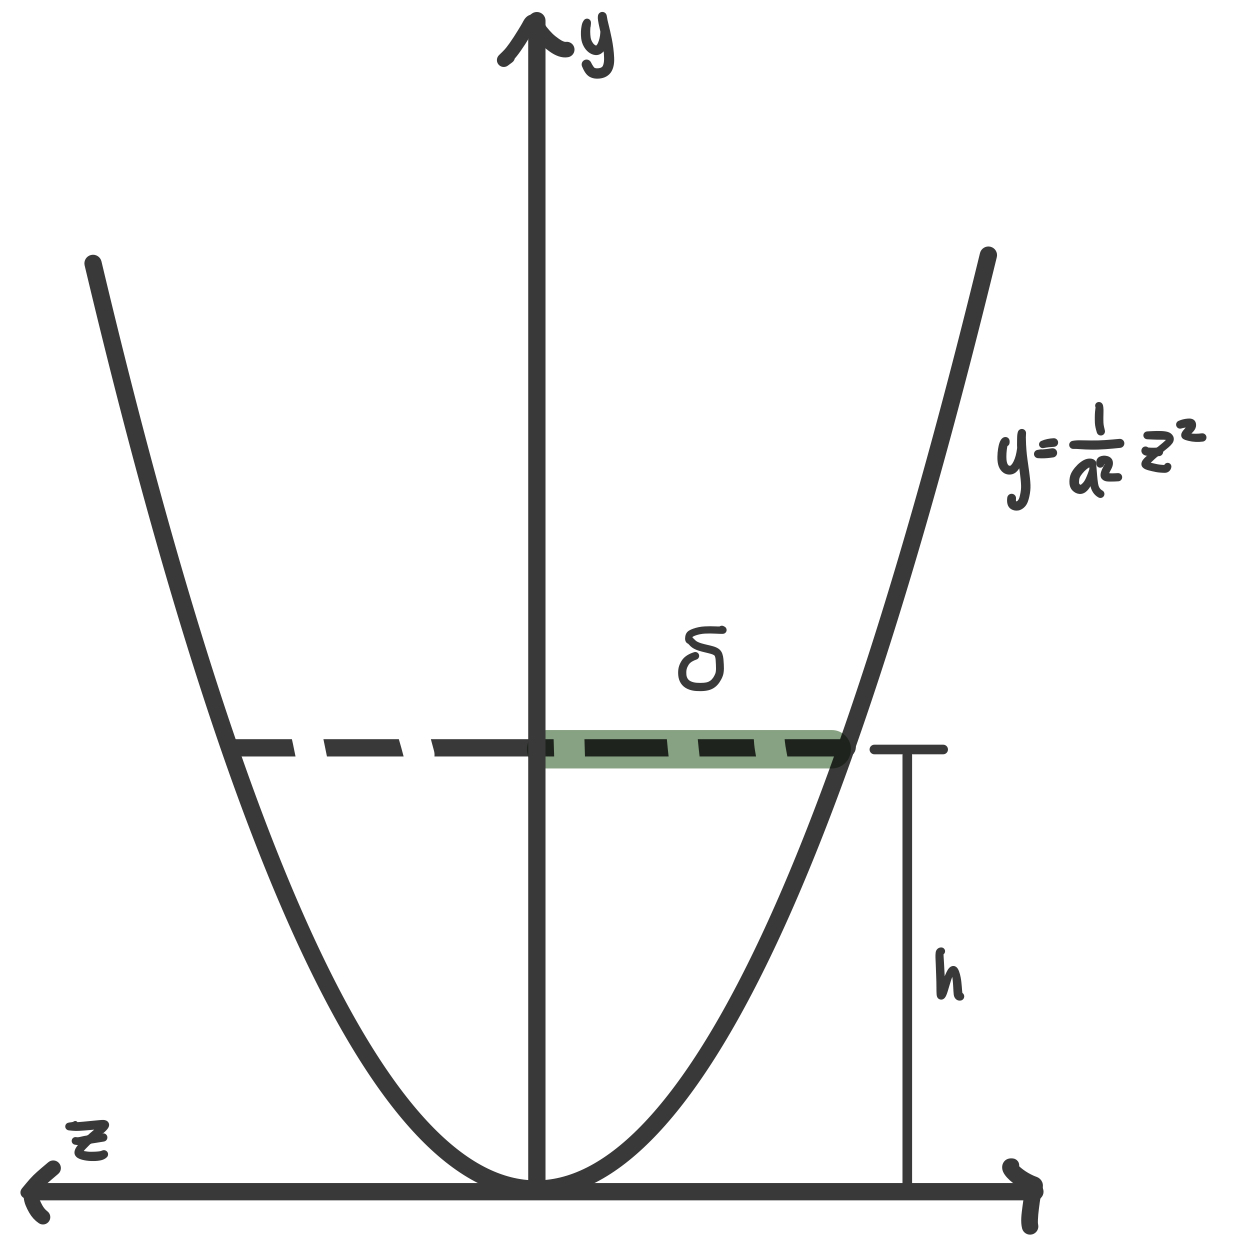
\includegraphics[width=0.6\textwidth]{more images/delta.jpg}
         \caption{Minor semi-axis length $z$-$y$ plane}
         \label{fig:zy}
     \end{subfigure}
     \hfill
        \caption{Analysing the semi-axes of the ellipse on 2-D planes}
        \label{fig:axes}
\end{figure}

We can get the length of the the major semi-axis, $\gamma$, by substituting it into the equation of the parabola that  ($\gamma$,$h$) is a point on as shown below:

$$
\begin{array}{l|c}
    y = \frac{1}{b^2}x^2 & \text{Parabola in the same axes} \\ \\
    (h) = \frac{1}{b^2}(\gamma)^2 & \text{Substituting } (\gamma, h) \\ \\
    \gamma^2 = b^2 h & \text{Making } \gamma \text{ the subject} \\ \\
 \end{array}
$$

\begin{equation}\label{solve.gammaparab}
    \boxed{\gamma = b\sqrt{h}}  \quad \text{Solving for } \gamma
\end{equation}

The same idea applies for the length $\delta$ of the semi-minor axis, where $\delta$ is the length across the $z$-axis, $h$ is the height along the $y$-axis, and ($\delta$,$h$) is a point on the parabola $y=\frac{1}{a^2}x^2$. By the same principle, we can say:

$$
\begin{array}{l|c}
    y = \frac{1}{\alpha^2}x^2 & \text{Parabola in the same axes} \\ \\
    (h) = \frac{1}{a^2}(\delta)^2 & \text{Substituting } (\delta, h) \\ \\
    \delta^2 = a^2 h & \text{Making } \delta \text{ the subject} \\ \\
 \end{array}
$$

\begin{equation}\label{solve.delta}
    \boxed{\delta = a\sqrt{h}}  \quad \text{Solving for } \delta
\end{equation}

Given we have now found the major and minor axes of our ellipse in terms of the height of a cross sectional area on the elliptical paraboloid ($h$), and the parabolas the axes are bound by ($a$ and $b$), we can find the cross sectional area at any height. The area of an ellipse, where $\chi$ is the area, is the product of $\pi$, the major semi-axis ($a \sqrt{h}$), and the minor semi-axis ($b \sqrt{h}$), giving us:

\vspace{-8mm}

\begin{equation}\label{solve chi}
    \boxed{\chi = \pi a b h}
\end{equation}

Now that we have an expression for the elliptical cross sectional area, we can create any hypothetical shape that has an equal cross-sectional area and height to model it. For this elliptical paraboloid, a triangular prism with a right-angle isosceles triangle as its face is most intuitive (\citeauthor{bogomolny}). 

\begin{figure}[h]
     \centering
     \begin{subfigure}[b]{0.45\textwidth}
         \centering
         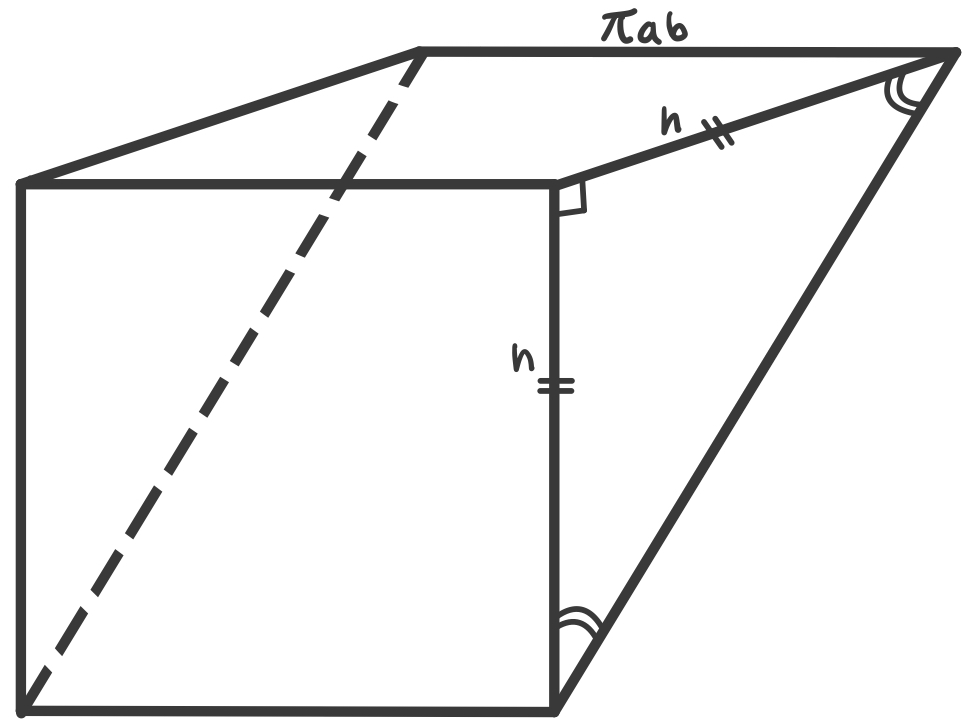
\includegraphics[width=0.6\textwidth]{more images/tria.jpg}
         \caption{Construction of triangular prism}
         \label{fig:full trig}
     \end{subfigure}
     \hfill
     \begin{subfigure}[b]{0.45\textwidth}
         \centering
         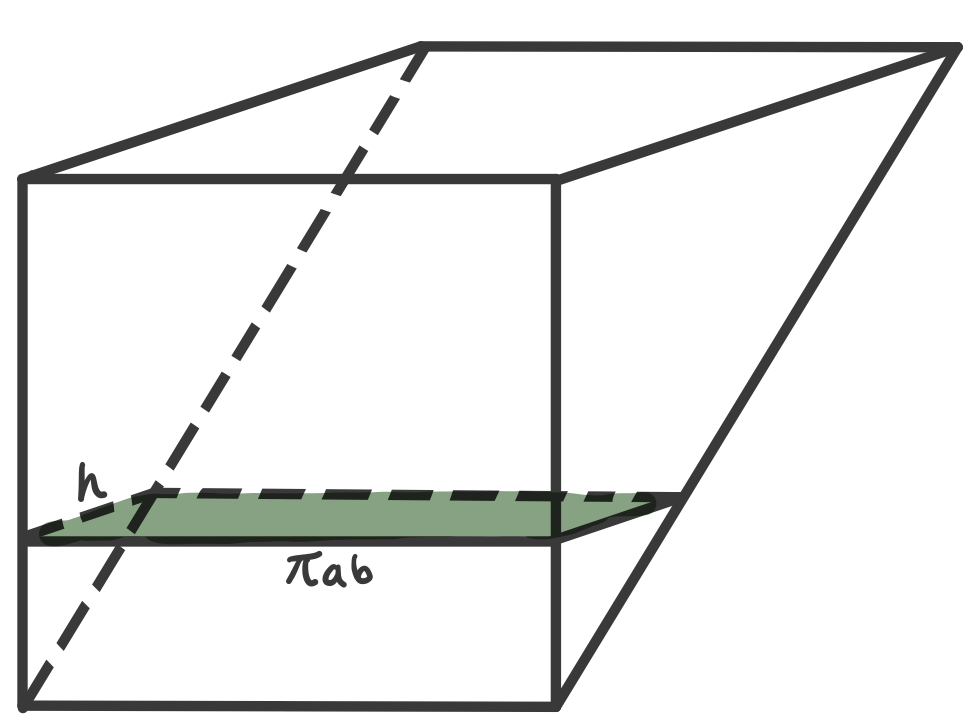
\includegraphics[width=0.6\textwidth]{more images/tria cross.jpg}
         \caption{Cross-sectional plane}
         \label{fig:cross trig}
     \end{subfigure}
     \hfill
        \caption{Creating the hypothetical shape}
        \label{fig:axes}
\end{figure}

The two congruent legs of the isosceles can have a length of $h$ as illustrated in my drawing, Figure \ref{fig:full trig}, and the prism can have a depth of $\pi a b$. We can say that the depth is $\pi ab$ because when taking a cross-sectional area of this triangular prism, we get a rectangle of length $\pi ab$ and width $h$ (Figure \ref{fig:cross trig}), giving us a cross-sectional area of $\pi ab h$, which is equal to that of the ellipse as calculated in Equation \ref{solve chi}. Since this triangular prism has the same height and cross-sectional area as our elliptical paraboloid, their volumes will be equal, as per Cavalieri's Principle.

Hence, we can calculate the volume, $V$ of our paraboloid by finding the volume of the triangular prism as follows:

$$
\begin{array}{l|c}
    V = (\text{area}) \times (\text{depth}) & \text{Volume formula} \\ \\
    V = \frac{hh}{2} \times \pi ab & \text{Substitute triangle area and depth} \\ \\
 \end{array}
$$

\begin{equation}\label{volume}
    \boxed{V = \frac{\pi a b h^2}{2}}  \quad \text{Arriving at}
\end{equation}

Now that we've found an equation for the volume of our paraboloid in terms of two parabolas and its height, we simply have to put our parabolas found earlier, $p(x)$ and $w(x)$, in the same form to find $a$ and $b$, and we can find the volume of our teaspoon.

We can start with $p(x)=0.0451x^2$ from Equation \ref{p(x)} where we want to find the $a$ value of that parabola in terms of $y=\frac{1}{a}x^2$ for our volume formula.

$$
\begin{array}{l|c}
    p(x) = \frac{1}{a^2}x^2 & \text{Parabola equivalency} \\ \\
    0.0451x^2 = \frac{1}{a^2}x^2 & \text{Substituting } p(x) \\ \\
    a = \sqrt{ \frac{x^2}{0.0451x^2}} & \text{Making } a \text{ the subject} \\ \\
 \end{array}
$$

\begin{equation}\label{solve.a!}
    \boxed{a = 4.7088}  \quad \text{Arriving at}
\end{equation}

We can carry out the same process for $w(x)$ from Equation \ref{w(x)} to find the $b$ value (process not be shown to maintain conciseness):

\begin{equation}\label{solve.b!}
    \boxed{b = 3.1879}
\end{equation}

Hence, using our formula for the volume of an elliptical paraboloid (Equation \ref{volume}), we can substitute in our $a$, $b$ and known height value, $h$ in and find the volume, $V$ of our teaspoon:

$$
\begin{array}{l|c}
    V = \frac{\pi a b h^2}{2} & \text{Volume formula} \\ \\
    V = \frac{\pi (4.7088)(3.1879)(0.8)^2}{2} & \text{Substituting } a, b \text{ and } h \\ \\
 \end{array}
$$

\begin{equation}\label{solve.a!}
    \boxed{V = 15.0909}  \quad \text{Arriving at}
\end{equation}


\section{Conclusion}

We find that through Cavalieri's Principle, the volume of my teaspoon is 15.0909 $cm^3$, or 15.0909 mL. After weighing the volume of my teaspoon on a scale (adjusted for volume of water $\pm 0.5$ mL), I found that the volume was 6 mL. There is a large discrepancy, specifically a 151.5 \% difference, as calculated below (Equation \ref{percentdif}). 

$$
\begin{array}{l|c}
    \% \text{ difference} = \frac{\text{theoretical} - \text{actual}}{\text{actual}} \times 100 & \text{\% difference formula} \\ \\
    \% \text{ difference} = \frac{15.0909 - 6}{6} \times 100 & \text{Substituting values} \\ \\
 \end{array}
$$

\begin{equation}\label{percentdif}
    \boxed{\% \text{ difference} = 151.5 \%}  \quad \text{Arriving at}
\end{equation}

The most likely reason for this discrepancy is the fact that the thickness of the spoon itself was not accounted for in any of the measurements. As the teaspoon was very small, the difference between the actual measurements and those with the thickness considered would be significant, causing all the values calculated to be higher than in reality. Additionally, a small error was introduced by rounding, which accumulated with each subsequent calculation. For example, this was evident when the calculated integrals for the transformed parabolas differed slightly from the integrals of the original equations. The assumption that the curves could be modelled by parabolas instead of finding an exact function of a higher degrees that modelled the curves also made the results significantly less accurate by not modelling the curves precisely. 

Nonetheless, I still found Cavalieri's Principle very interesting as it relies heavily on the intuitive nature of mathematics. I thought it to be a perfect demonstration of how mathematics can be beautiful, especially when we arrived at the final equation for the volume of an elliptical paraboloid, being an unexpected simple solution. A strength of using Cavalieri's Principle is that it allows us to solve for the volume of complex shapes without using multi-variable calculus, but rather intuitive geometry. This not only allows problems to have simpler and easier to understand solutions, but also be applied in numerous contexts. I believe Cavalieri's Principle would be much more effective when measuring large objects, where small error that is introduced wouldn't have as great of an effect on the overall volume as it did in this investigation.

An interesting extension would of course be using multi-variable calculus to solve this problem. It would be quite interesting to see what the difference is when using the exact same numbers to see how much error all the transforming of parabolas introduced when using Cavalieri's Principle. However, it would also be interesting to see how close we could get to the actual volume of the teaspoon given the right measurements using Cavalieri's Principle, and if perhaps there is a better shape that the elliptical paraboloid could've been transformed onto, or if assuming an elliptical paraboloid modelled the teaspoon was incorrect.

Overall, I now know that my teaspoon is just over a US standard teaspoon, which measures 4.9289 mL whereas mine is 6 mL. Albeit I did not conclude this information from the investigation itself, I did find it out as a result of it. I think the biggest lesson however, was learning how there are always different methods in mathematics. When I was confronted by the possibility of multi-variable calculus, I thought my investigation was going to be too complex, but through an intuitive geometrical approach, I was able to solve that very problem.



\pagebreak

\printbibliography

\end{document}